\documentclass{article}

\usepackage[math,lf,footnotefigures]{MyriadPro}
\renewcommand{\familydefault}{\sfdefault}
\newcommand*{\mytextstyle}{\sffamily\Large\bfseries\color{black!85}}
%\usepackage[T1]{fontenc}

\usepackage{tikz}
\usetikzlibrary{arrows}
\usetikzlibrary{arrows.meta}
\usetikzlibrary{positioning}
\usetikzlibrary{decorations.text}

\usepackage{xcolor}
\definecolor{ufzgray1}{RGB}{126,126,126}
\definecolor{ufzgray2}{RGB}{156,156,156}
\definecolor{ufzgray3}{RGB}{185,185,185}
\definecolor{ufzgray4}{RGB}{230,230,230}

\usepackage{enumitem}

% adjust the page margins
\usepackage[left=2.7cm,right=2.5cm,top=1.2cm,bottom=1cm]{geometry}

% arc arrows
% arc arrows
\newcommand{\arcarrow}[3]{%
	% inner radius, middle radius, outer radius, start angle,
	% end angle, tip protusion angle, options, text
	\pgfmathsetmacro{\rin}{1.7}
	\pgfmathsetmacro{\rmid}{2.2}
	\pgfmathsetmacro{\rout}{2.7}
	\pgfmathsetmacro{\astart}{#1}
	\pgfmathsetmacro{\aend}{#2}
	\pgfmathsetmacro{\atip}{5}
	\fill[ufzgray1!10, very thick] (\astart-\atip:\rin)
	arc (\astart-\atip:\aend:\rin)
	-- (\aend+\atip:\rmid)
	-- (\aend:\rout)   arc (\aend:\astart-\atip:\rout)
	-- (\astart:\rmid) -- cycle;
	\path[
	decoration = {
		text along path,
		text = {|\mytextstyle|#3},
		text align = {align = center},
		raise = -1.0ex
	},
	decorate
	](\astart+\atip:\rmid) arc (\astart+\atip:\aend+\atip:\rmid);
}

% cloud
\usetikzlibrary{calc}
\newcommand{\AsymCloud}[3]{
	\begin{scope}[shift={#1},scale=#3,color=ufzgray1]
		\draw (-1.6,-0.7) .. controls (-2.3,-1.1)
		and (-2.7,0.3) .. (-1.7,0.3)coordinate(asy1) .. controls (-1.6,0.7)
		and (-1.2,0.9) .. (-0.8,0.7) .. controls (-0.5,1.5)
		and (0.6,1.3) .. (0.7,0.5) .. controls (1.5,0.4)
		and (1.2,-1) .. (0.4,-0.6)coordinate(asy2) .. controls (0.2,-1)
		and (-0.2,-1) .. (-0.5,-0.7) .. controls (-0.9,-1)
		and (-1.3,-1) .. cycle;
		\node[align=center,yshift=0.1cm] at ($(asy1)!0.5!(asy2)$) {#2};
	\end{scope}
}

\begin{document}
	
	\pagestyle{empty}
	
	\hspace*{-3cm}
	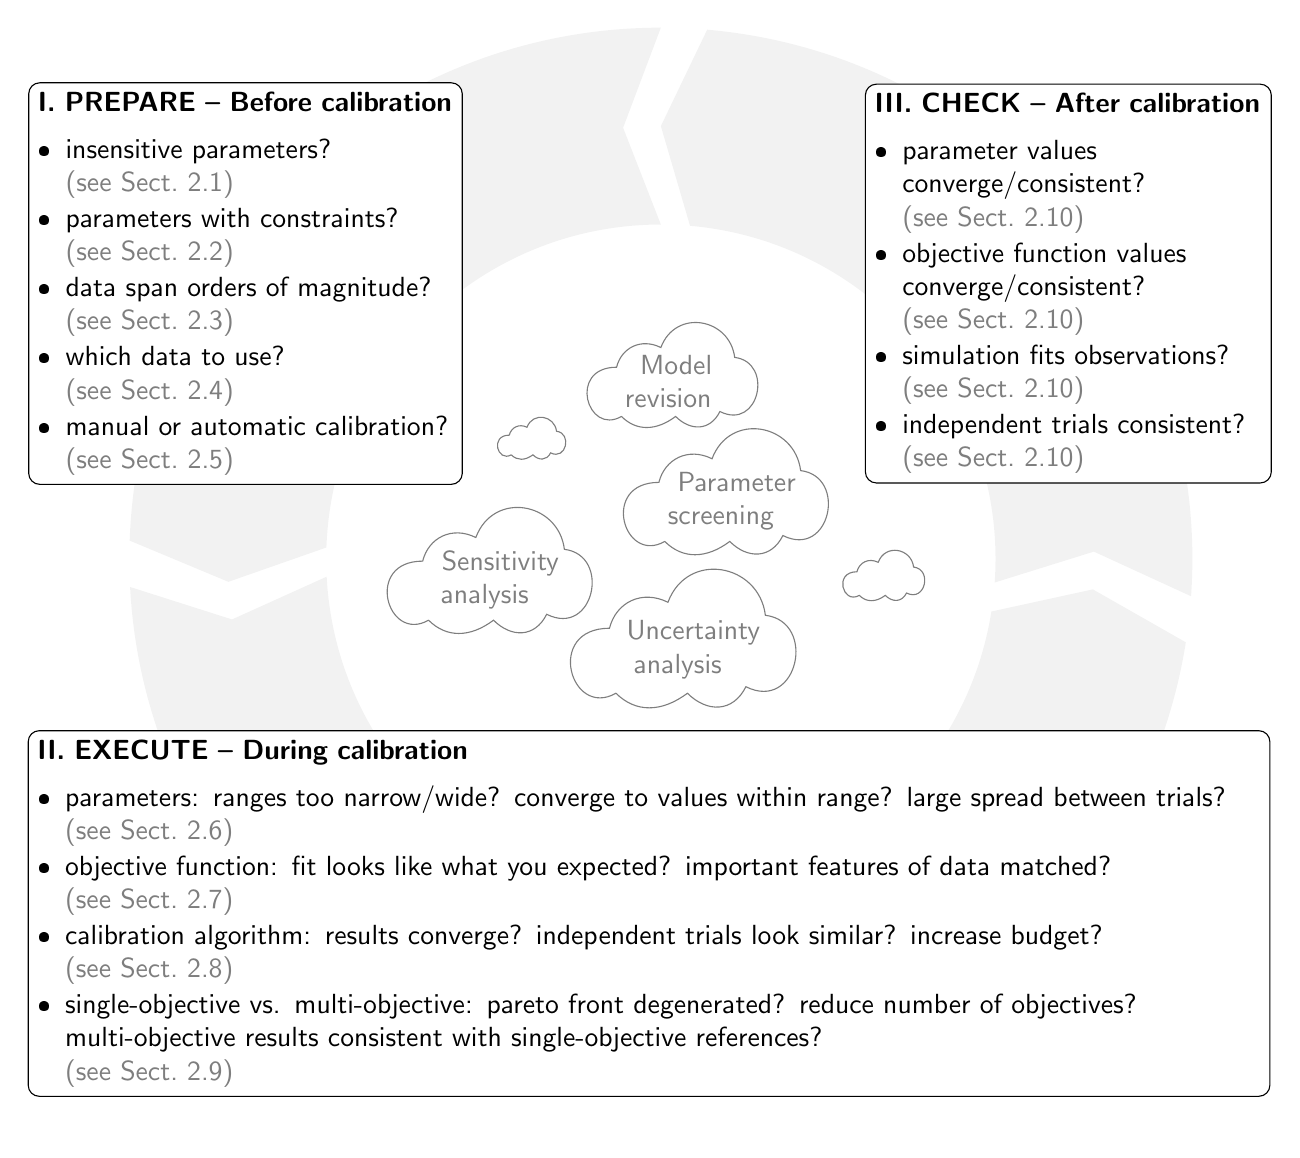
\begin{tikzpicture}[scale=2.5]
	
		\tikzstyle{block} = [rectangle, draw, fill=white!20, text centered, rounded corners, minimum height=1em]
		\tikzstyle{blockwide} = [rectangle, draw, fill=white!20, 
		text width=14.5em, text centered, rounded corners, minimum height=1em]
		\tikzstyle{noblock} = [rectangle, %fill=white!20, 
		text width=27.0em, rounded corners, minimum height=1em]
		\tikzstyle{noblockwide} = [rectangle, %fill=white!20, 
		text width=14.5em, rounded corners, minimum height=1em]
		\tikzstyle{abcblock} = [rectangle, fill=white!20, 
		text width=1em, rounded corners, minimum height=1em]
		\tikzstyle{line} = [draw, -latex']
		\tikzstyle{line} = [draw,latex'-latex'new]
		
		% arrows
		% found at: https://texample.net/tikz/examples/pdca-cycle/
		\arcarrow{1}{85}{ }
		\arcarrow{ 95}{178}{ }
		\arcarrow{188}{351}{ }
		
		% clouds
		\pgfmathsetmacro{\cloudxshift}{-0.1}
		\pgfmathsetmacro{\cloudyshift}{-0.4}
		\AsymCloud{(-0.5+\cloudxshift,1.0+\cloudyshift)}{}{0.1}
		\AsymCloud{(1.3+\cloudxshift,0.3+\cloudyshift)}{}{0.12}
		\AsymCloud{(0.3+\cloudxshift,1.3+\cloudyshift)}{\hspace*{0.2cm}Model\\revision}{0.25}
		\AsymCloud{(0.6+\cloudxshift,0.7+\cloudyshift)}{\hspace*{0.4cm}Parameter\\screening}{0.3}
		\AsymCloud{(-0.6+\cloudxshift,0.3+\cloudyshift)}{\hspace*{0.4cm}Sensitivity\\analysis}{0.3}
		\AsymCloud{(0.4+\cloudxshift,-0.05+\cloudyshift)}{\hspace*{0.4cm}Uncertainty\\analysis}{0.33}
	
		% start
		\node [block,text width=15em,align=left,xshift=3.8cm] at (-3.63,1.4) {\hspace*{0.0cm}\textbf{I. PREPARE~--~Before calibration}\vspace*{-0.3em}
			\hspace*{-0.6cm}
			\begin{itemize}[leftmargin=*]
				\setlength\itemsep{-0.3em}
				\item insensitive parameters?\\ \textcolor{ufzgray1}{(see Sect.~2.1)} %consider fixing insensitive parameters during calibrating or avoid reporting their ``calibrated'' values\\ 
				\item parameters with constraints?\\ \textcolor{ufzgray1}{(see Sect.~2.2)}
				\item data span orders of magnitude?\\ \textcolor{ufzgray1}{(see Sect.~2.3)}
				\item which data to use?\\ \textcolor{ufzgray1}{(see Sect.~2.4)}
				\item manual or automatic calibration?\\ \textcolor{ufzgray1}{(see Sect.~2.5)}
		\end{itemize}};
		
		% do
		\node [block,text width=44.2em,align=left,xshift=3.8cm] at (-1.58,-1.8) {\hspace*{0.0cm}\textbf{II. EXECUTE~--~During calibration}\vspace*{-0.3em}
			\hspace*{-0.6cm}
			\begin{itemize}[leftmargin=*]
				\setlength\itemsep{-0.3em}
				\item parameters: ranges too narrow/wide? converge to values within range? large spread between trials?\\ \textcolor{ufzgray1}{(see Sect.~2.6)}
				\item objective function: fit looks like what you expected? important features of data matched?\\ \textcolor{ufzgray1}{(see Sect.~2.7)}
				\item calibration algorithm: results converge? independent trials look similar? increase budget?\\ \textcolor{ufzgray1}{(see Sect.~2.8)}
				\item single-objective vs. multi-objective: pareto front degenerated? reduce number of objectives? multi-objective results consistent with single-objective references?\\ \textcolor{ufzgray1}{(see Sect.~2.9)}
				
		\end{itemize}};
		
		% check
		\node [block,text width=14em,align=left,xshift=3.8cm] at (0.55,1.4) {\hspace*{0.0cm}\textbf{III. CHECK~--~After calibration}\vspace*{-0.3em}
			\hspace*{-0.6cm}
			\begin{itemize}[leftmargin=*]
				\setlength\itemsep{-0.3em}
				\item parameter values converge/consistent?\\ \textcolor{ufzgray1}{(see Sect.~2.10)}
				\item objective function values converge/consistent?\\ \textcolor{ufzgray1}{(see Sect.~2.10)}
				\item simulation fits observations?\\ \textcolor{ufzgray1}{(see Sect.~2.10)}
				\item independent trials consistent?\\ \textcolor{ufzgray1}{(see Sect.~2.10)}
		\end{itemize}};
				
	\end{tikzpicture}
	
\end{document}



